
\section{Reconnaissance des entités nommées}
La reconnaissance des entités nommées s'effectue au sein des sections correspondant aux textes des rentes qui sont stockées dans le tableau de données principal. Chacune de ces sections est fouillée à l'aide d'une expression régulière afin de détecter les caractéristiques morphosyntaxiques correspondant aux anthroponymes du  nord  de la France au Moyen-Âge.
\newpage
L'expression régulière dont il est question nous est donnée par les travaux de S. De Valeriola\footfullcite[p.10]{de_valeriola_lordinateur_2021}. À celle-ci, un petit ajout a été effectué afin de capturer les éventuelles abréviations <<Mgr>>  ---  correspondant au titre de <<Monseigneur>> --- qui, si elles ne sont pas prises en considération, empêchent ponctuellement l'expression régulière de capturer l'entièreté de l'anthroponyme.

\[
    \boxed{
        \begin{array}{c}
        \textit{(Mgr)\;?[:upper:][:lower:]+\;(((l[aei']s?|d[euo']l?u?|au?)?)\{0,2\} \;?}\\
        \textit{[:upper:][:lower:]+(-[:upper:][:lower:]+)?)\{1,3\}}
        \end{array}
    }
\]

Celle-ci peut être décomposée en quatre sous-expressions, correspondant chacune à une partie de l'anthroponyme.
\begin{itemize}
    \item La première partie capture le titre  dans l'éventualité où il y en a un : \[(Mgr)\; ?\]
    \item La seconde capture le nom de baptême de la personne : \[[:upper:][:lower:]+\]
    \item La troisième permet de capturer les éventuelles particules de patronyme ( par exemple : <<de>>, <<dou>>, <<le>>, <<l'>> , <<de le>>, etc.) : \[ ((l[aei']s?|d[euo']l?u?|au?)?)\{0,2\}\;?\] 
    \item Finalement, la dernière partie sert à capturer le reste du patronyme, sans les éventuelles particules : \[[:upper:][:lower:]+(-[:upper:][:lower:]+)?)\{1,3\}\] 
\end{itemize}

Grâce à cette expression régulière, la fonction \textit{str\_extract\_all()} de la bibliothèque \textit{StringR} nous retourne 799 formes distinctes d'anthroponyme. 


\subsection{Déterminer la stratégie de regroupement}
%choix de la méthode de clustering
Comme  il en a été discuté dans le chapitre \textit{Méthodes}, le choix de la méthode et de la distance de seuil pour le regroupement des anthroponymes est une étape aussi critique que délicate.
Afin de choisir la stratégie la plus adéquate, des tests ont été effectués sur les 100 premiers anthroponymes, noms de baptême et patronymes recensés dans le document source.

%modalités des tests
À travers ces tests, il a été observé la dispersion des groupes, corrects et incorrects, déterminés par l'algorithme en fonction de la distance, l'évolution du taux de bruit en fonction de la distance, et l'impact, positif ou négatif, d'une modification de pondération des opérations\footnote{Cette modification de pondération s'ajoute à celles évoquées dans le chapitre \textit{Méthodes} provenant de l'article de \fullcite[p.14]{de_valeriola_lordinateur_2021}} dans le calcul de la distance.
Cette modification de pondération consiste à passer le poids des opérations de substitution de 1,0 à 1,25.
%justification de la modification de pondération
L'idée derrière cette modification est d'alourdir significativement le score lorsque plusieurs opérations de substitution sont utilisées. 
Étant donné que la plupart des variants morphologiques d'un anthroponyme consistent en l'ajout ou la suppression d'une lettre ou d'une particule, les opérations de substitution sont relativement rares et ont un impact plus lourd que les autres opérations sur la modification de la chaîne de caractères.

%methode
La distance Damerau-Levensthein entre chaque nom testé est calculée, et tous les couples de noms dont la distance est égale ou inférieure à la distance de seuil (changeante en fonction de la nature des éléments testés) sont regroupés dans un tableau de données. Après quoi, chaque groupe est manuellement vérifié et annoté <<correct>> ou <<incorrect>> par l'agent humain.

Six configurations ont donc été analysées :
\begin{itemize}
    \item sur l'anthroponyme complet (nom de baptême et patronyme), considéré comme une seule chaîne de caractères, avec une distance de seuil à 3 (tableau \ref{groupe_anthro}).
    \item Sur l'anthroponyme complet, avec une distance de seuil à 4, et avec la modification de la pondération (tableau \ref{groupe_anthro_md}).
    \item Sur le nom de baptême uniquement, avec une distance de seuil à 2 (tableau \ref{groupe_prenom}).
    \item Sur le nom de baptême uniquement, avec une distance de seuil à 2, et avec la modification de pondération (tableau \ref{groupe_prenom_md}).
    \item Sur le patronyme uniquement, avec une distance de seuil à 3 (tableau \ref{groupe_patro}).
    \item Sur le patronyme,avec une distance de seuil à 3, et avec la modification de pondération (tableau \ref{groupe_patro_md}).
\end{itemize}
\vspace{0,5cm}



\renewcommand{\arraystretch} {1.25}
\begin{table}[ht]
    \centering
    \begin{tabular}{|c|c|c|c|c|c|c|c|}
        \hline \multicolumn{2}{|c}{D = 1}& \multicolumn{2}{|c}{D = 2} & \multicolumn{2}{|c}{D = 3} & \multicolumn{2}{|c|}{D = 4} \\
        \hline VRAI & FAUX & VRAI & FAUX & VRAI & FAUX & VRAI & FAUX \\
        \hline \hline  8 & 0 & 0 & 0 & 2 & 0 & 0 & 22 \\
        \hline 25\% & 0\% & 0\% & 0\% & 6\% & 0\% & 0\% & 69\%  \\
        \hline \hline \multicolumn{2}{|c}{Nb cum = 8 }& \multicolumn{2}{|c|}{Nb cum = 8 } & \multicolumn{2}{c|}{Nb cum = 10} & \multicolumn{2}{c|}{Nb cum = 32} \\
        \hline \hline  8 & 0 & 8 & 0 & 10 & 0 & 10 & 22 \\
        \hline 100\% & 0\% & 100\% & 0\% & 100\% & 0\% & 31\% & 69\%  \\
        \hline 
    \end{tabular}
    \caption{Analyse sur le groupe de test des anthroponymes }
    \label{groupe_anthro}
\end{table}

\renewcommand{\arraystretch} {1.25}
\begin{table}[ht]
    \centering
    \begin{tabular}{|c|c|c|c|c|c|c|c|}
        \hline \multicolumn{2}{|c}{D = 1}& \multicolumn{2}{|c}{D = 2} & \multicolumn{2}{|c}{D = 3} & \multicolumn{2}{|c|}{D = 4} \\
        \hline VRAI & FAUX & VRAI & FAUX & VRAI & FAUX & VRAI & FAUX \\
        \hline \hline  8 & 0 & 0 & 0 & 2 & 0 & 0 & 0 \\
        \hline 80\% & 0\% & 0\% & 0\% & 20\% & 0\% & 0\% & 0\%  \\
        \hline \hline \multicolumn{2}{|c}{Nb cum = 8}& \multicolumn{2}{|c|}{Nb cum = 8} & \multicolumn{2}{c|}{Nb cum = 10} & \multicolumn{2}{c|}{Nb cum = 10} \\
        \hline \hline  8 & 0 & 8 & 0 & 10 & 0 & 10 & 22 \\
        \hline 100\% & 0\% & 100\% & 0\% & 100\% & 0\% & 100\% & 0\%  \\
        \hline 
    \end{tabular}
    \begin{center}
        \caption{Analyse sur le groupe  de test des anthroponymes avec modification de pondération}
    \end{center}
    
    \label{groupe_anthro_md}
\end{table}

\renewcommand{\arraystretch} {1.25}
\begin{table}[ht]
    \centering
    \begin{tabular}{|c|c|c|c|}
        \hline \multicolumn{2}{|c}{D = 1}& \multicolumn{2}{|c|}{D = 2}\\
        \hline VRAI & FAUX & VRAI & FAUX \\
        \hline \hline  21 & 5 & 5 & 49 \\
        \hline 26\% & 6\% & 6\% & 61\% \\
        \hline \hline \multicolumn{2}{|c}{Nb cum = 26}& \multicolumn{2}{|c|}{Nb cum = 80}\\
        \hline \hline  21 & 5 & 26 & 54 \\
        \hline 81\% & 19\% & 33\% & 68\% \\
        \hline 
    \end{tabular}
    \caption{Analyse sur le groupe  de test des noms de baptême}
    \label{groupe_prenom}
\end{table}

\renewcommand{\arraystretch} {1.25}
\begin{table}[ht]
    \centering
    \begin{tabular}{|c|c|c|c|c|c|c|c|}
        \hline \multicolumn{2}{|c}{D = 1}& \multicolumn{2}{|c|}{D =2 }\\
        \hline VRAI & FAUX & VRAI & FAUX \\
        \hline \hline  18 & 0 & 2 & 6 \\
        \hline 53\% & 0\% & 6\% & 18\% \\
        \hline \hline \multicolumn{2}{|c}{Nb cum = 18}& \multicolumn{2}{|c|}{Nb cum = 34}\\
        \hline \hline  18 & 0 & 25 & 9 \\
        \hline 100\% & 0\% & 74\% & 26\% \\
        \hline 
    \end{tabular}
    \caption{Analyse sur le groupe de test des noms de baptême avec modification de pondération}
    \label{groupe_prenom_md}
\end{table}
\vspace{1cm}

\renewcommand{\arraystretch} {1.25}
\begin{table}[ht]
    \centering
    \begin{tabular}{|c|c|c|c|c|c|}
        \hline \multicolumn{2}{|c}{D = 1}& \multicolumn{2}{|c}{D = 2} & \multicolumn{2}{|c|}{D = 3 } \\
        \hline VRAI & FAUX & VRAI & FAUX & VRAI & FAUX \\
        \hline \hline  12 & 4 & 0 & 14 & 0 & 78 \\
        \hline 11\% & 4\% & 0\% & 13\% & 0\% & 72\% \\
        \hline \hline \multicolumn{2}{|c}{Nb cum = 16}& \multicolumn{2}{|c|}{Nb cum = 30} & \multicolumn{2}{c|}{Nb cum = 108} \\
        \hline \hline  12 & 4 & 12 & 18 & 12 & 96 \\
        \hline 75\% & 25\% & 40\% & 60\% & 11\% & 89\% \\
        \hline 
    \end{tabular}
    \caption{Analyse sur le groupe de test des patronymes }
    \label{groupe_patro}
\end{table}

\renewcommand{\arraystretch} {1.25}
\begin{table}[ht]
    \centering
    \begin{tabular}{|c|c|c|c|c|c|c|c|}
        \hline \multicolumn{2}{|c}{D = 1}& \multicolumn{2}{|c}{D = 2} & \multicolumn{2}{|c|}{D = 3} \\
        \hline VRAI & FAUX & VRAI & FAUX & VRAI & FAUX \\
        \hline \hline  11 & 1 & 0 & 2 & 2 & 6 \\
        \hline 29\% & 3\% & 0\% & 5\% & 5\% & 16\% \\
        \hline \hline \multicolumn{2}{|c}{Nb cum = 12}& \multicolumn{2}{|c|}{Nb cum = 18} & \multicolumn{2}{c|}{Nb cum = 38} \\
        \hline \hline  11 & 1 & 11 & 7 & 13 & 25 \\
        \hline 92\% & 8\% & 61\% & 39\% & 34\% & 66\% \\
        \hline 
    \end{tabular}
    \caption{Analyse sur le groupe de test des patronymes avec modification de pondération}
    \label{groupe_patro_md}
\end{table}

\begin{figure}[ht] % insère une figure ici (h = "here")
    \centering
    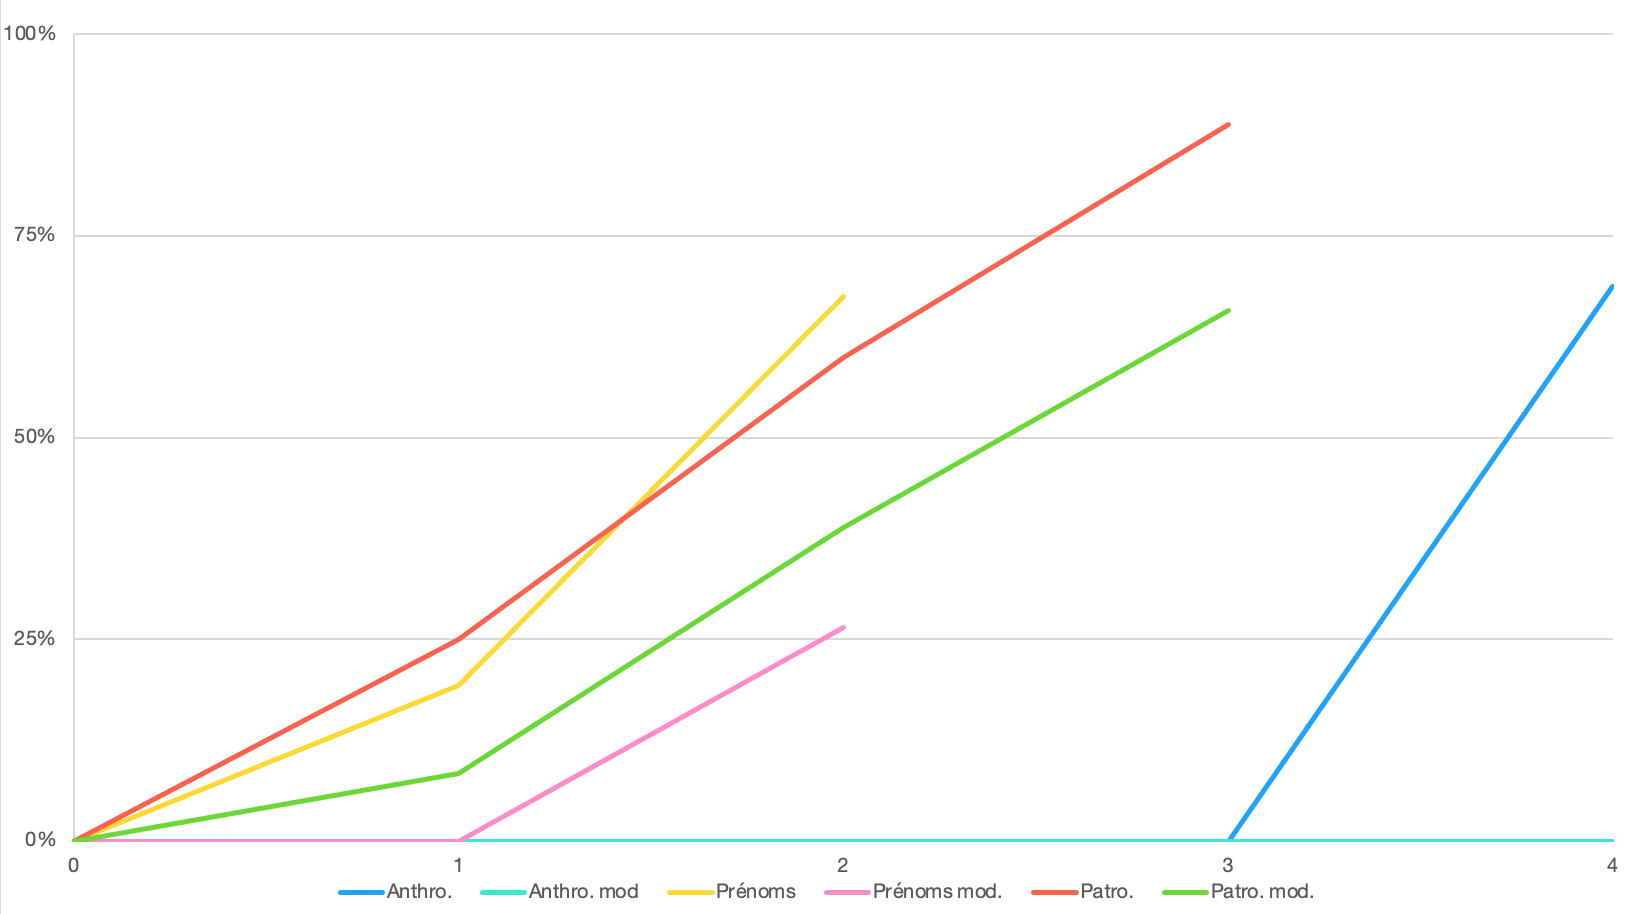
\includegraphics[scale=0.5]{3.Results/Img/noise_rate.png}
    \caption{Comparatif quant à l'évolution du bruit en fonction de la distance}
    \label{graph_methode_cluster}
\end{figure}

\begin{figure}[ht] % insère une figure ici (h = "here")
    \centering
    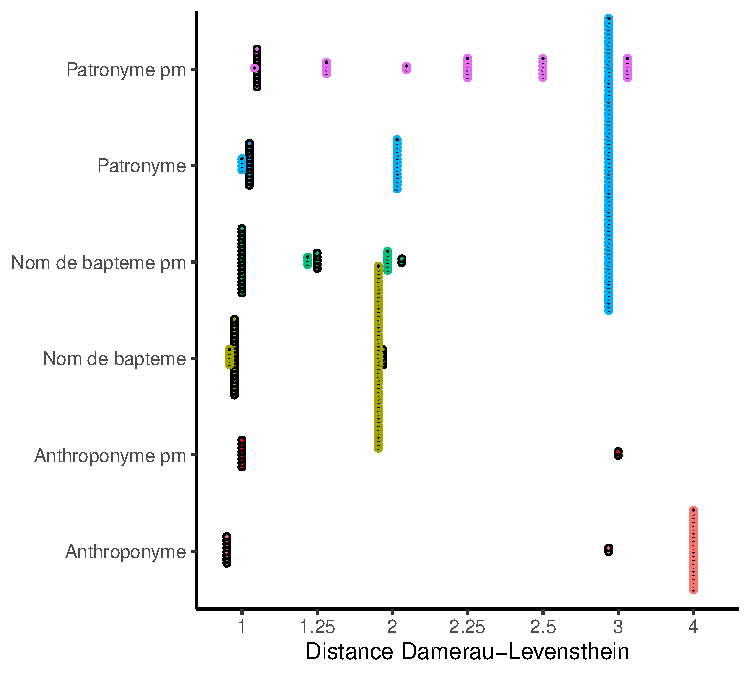
\includegraphics[scale=1.2]{3.Results/Img/Dotplot.pdf}
    \caption{Dispersion des couples en fonction de la distance}
    \label{graph_dispertion_cluster}
\end{figure}

On observe un résultat peu surprenant à certains égards : les groupes corrects sont principalement ceux ayant des éléments séparés par une faible distance, et la grande majorité des couples incorrects sont ceux dont les éléments sont séparés par une grande distance. 
Plus les chaînes de caractères sont, en moyenne, longues, plus ce phénomène se marque.
Ainsi, dans les noms de baptême, qui sont généralement plus courts que les patronymes ou les anthroponymes, on observe du bruit, et ce même dans les groupes à une distance de 1. Alors que dans les anthroponymes on retrouve les premières traces de bruit qu’à partir de 4 distances.
Une autre observation est que le changement de pondération améliore notablement la justesse des résultats --- entre 17 \% et 40 \% d'amélioration  --- pour tous les . Pour être plus exacte, la modification diminue le taux de bruit sans pour autant affecter le taux de rappel.
Ce sont donc les tests sur le groupe des anthroponymes entiers, avec l'alourdissement du poids des opérations de substitution à 1.25 au lieu de 1, et un seuil de distance à 3, qui retournent les meilleurs résultats avec une exactitude complète des groupes déterminés depuis l'échantillon de test.

\subsection{Regroupement des anthroponymes}
%matrice de distance et heatmap
Le script qui regroupe des anthroponymes par le biais du calcul des distances Damerau-Levensthein est utilisé sur le vecteur contenant l'ensemble des formes d'anthroponymes recensés au sein du document source. L'opération est relativement lourde pour l'ordinateur puisqu'il a à calculer 638401 résultats au travers de celle-ci et prend, par conséquent, un certain temps. La figure \ref{heatmap_anthro} représente le graphique de type \textit{Heatmap} retourné par l'exécution du script. Celui-ci apporte une plus-value discutable dans l'analyse ou la détection des formes variantes des anthroponymes, mais a le mérite d'illustrer parfaitement l'impossibilité d'effectuer ces opérations manuellement, et, par extension, la nécessité de développer des processus automatisés pour résoudre ceux-ci.
\begin{figure}
    \centering
    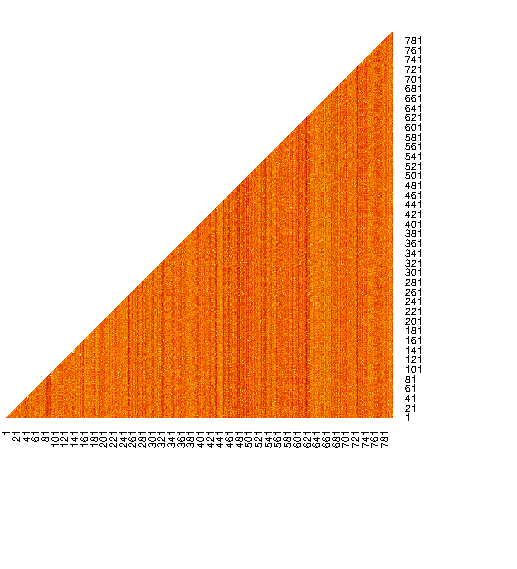
\includegraphics [scale=2]{3.Results/Img/heatmap.pdf}
    \caption{Heatmap des distances séparant chaque anthroponyme}
    \label{heatmap_anthro}
\end{figure}

%resultat
\subsection{Évaluation}
Bien que la stratégie choisie ait rendu des résultats encourageants sur le groupe de test, lorsqu'elle est appliquée à l'ensemble des anthroponymes du document source, ceux-ci ne sont plus aussi probants. L'algorithme détermine 74 groupes de deux à trois anthroponymes dans les 799 formes uniques recensées. Parmi ces groupes, seuls 46 sont parfaitement justes, tandis que 26 sont entièrement faux, et 2 sont partiellement faux ; soit 62 \% de justesse. Une correction par l'agent humain de cette liste avant que les formes variantes soient remplacées par une forme générale dans le tableau de données principal semble donc nécessaire afin de ne pas dégrader excessivement la qualité des données récoltées.
Le tableau \ref{clustering_corr} contenant les groupes déterminés par l'algorithme, ainsi que sa correction, est consultable dans la partie \textit{Annexes}.


